
%(BEGIN_QUESTION)
% Copyright 2006, Tony R. Kuphaldt, released under the Creative Commons Attribution License (v 1.0)
% This means you may do almost anything with this work of mine, so long as you give me proper credit

Beregn hydrostatisk trykk i bunnen av denne tanken (i bar) når den er helt fylt med vann:

$$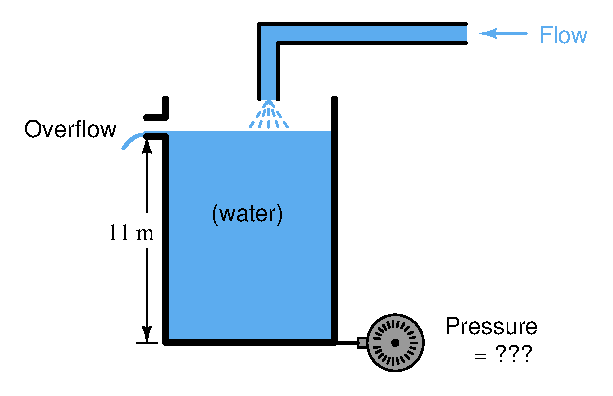
\includegraphics[height=6cm]{i00308x01.eps}$$

Beregn deretter hydrostatisk trykk i bunnen av tanken (i bar) når den er helt fylt med bensin (tetthet = 672.8 kg/m$^{3}$):

$$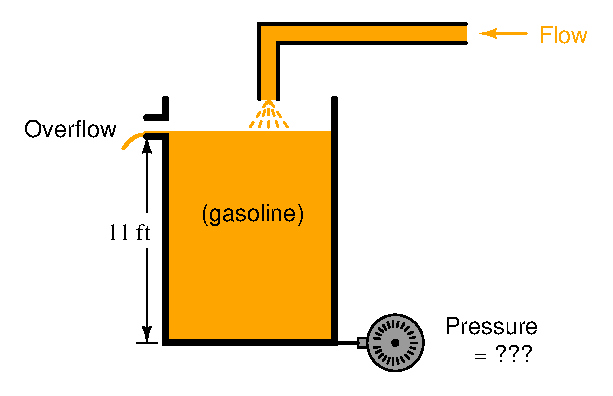
\includegraphics[height=6cm]{i00308x02.eps}$$

\filbreak

Hva tror du trykket i bunnen blir hvis tanken er nøyaktig halvfull med bensin og halvfull med vann, med bensin-vann-\textit{interface} ved 5.5 meter?  Forklar resonnementet.

$$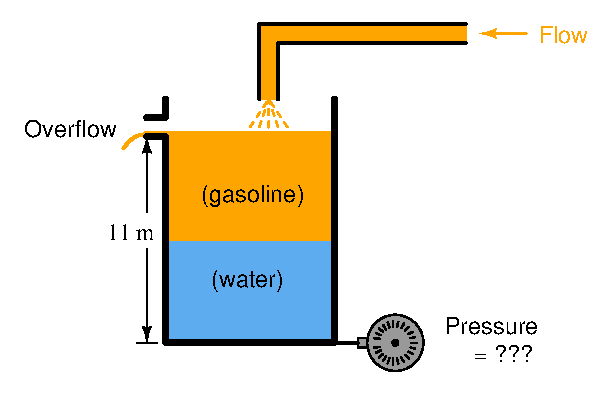
\includegraphics[height=6cm]{i00308x03.eps}$$

\underbar{file i00308}
%(END_QUESTION)





%(BEGIN_ANSWER)

Hydrostatisk trykk ved helt full av vann = 1.065 bar

\vskip 10pt

Hydrostatisk trykk ved helt full av bensin = 0.717 bar

\vskip 10pt

Hydrostatisk trykk når vann-bensin-grensesnitt ligger på 50\% nivå = 0.891 bar

%(END_ANSWER)





%(BEGIN_NOTES)


%INDEX% Physics, static fluids: hydrostatic pressure of liquid/liquid interface

%(END_NOTES)
